% Pipeline PaddleOCR-only. Tahapan mengikuti kode yang benar benar berjalan:
% featurize_image_blocks -> LogisticRegression -> predict_fields_geo.
% Kompilasi: pdflatex architecture-paddle.tex
\documentclass[border=14pt,tikz]{standalone}
\usepackage[T1]{fontenc}
\usepackage{tikz}
\usetikzlibrary{arrows.meta,positioning,fit,backgrounds,calc}
\pgfdeclarelayer{bgA}\pgfdeclarelayer{bgB}
\pgfsetlayers{bgB,bgA,main}

\definecolor{gGray}  {HTML}{E8EAED}
\definecolor{gBlueBg}{HTML}{DCEAFB}\definecolor{gBlue}  {HTML}{2E6DB4}\definecolor{gBlueLt}{HTML}{5B9BD5}
\definecolor{gPurBg} {HTML}{EFE4F7}\definecolor{gPur}   {HTML}{6B3FA0}
\definecolor{gPinkBg}{HTML}{FBE0E8}\definecolor{gPink}  {HTML}{B03A5B}
\definecolor{gOrange}{HTML}{C1610E}
\definecolor{gCream} {HTML}{FBF3DE}\definecolor{gTan}   {HTML}{A8871F}
\definecolor{gAmber} {HTML}{E8873C}
\definecolor{gEdge}  {HTML}{5F6368}
\definecolor{gMuted} {HTML}{80868B}

\begin{document}\sffamily
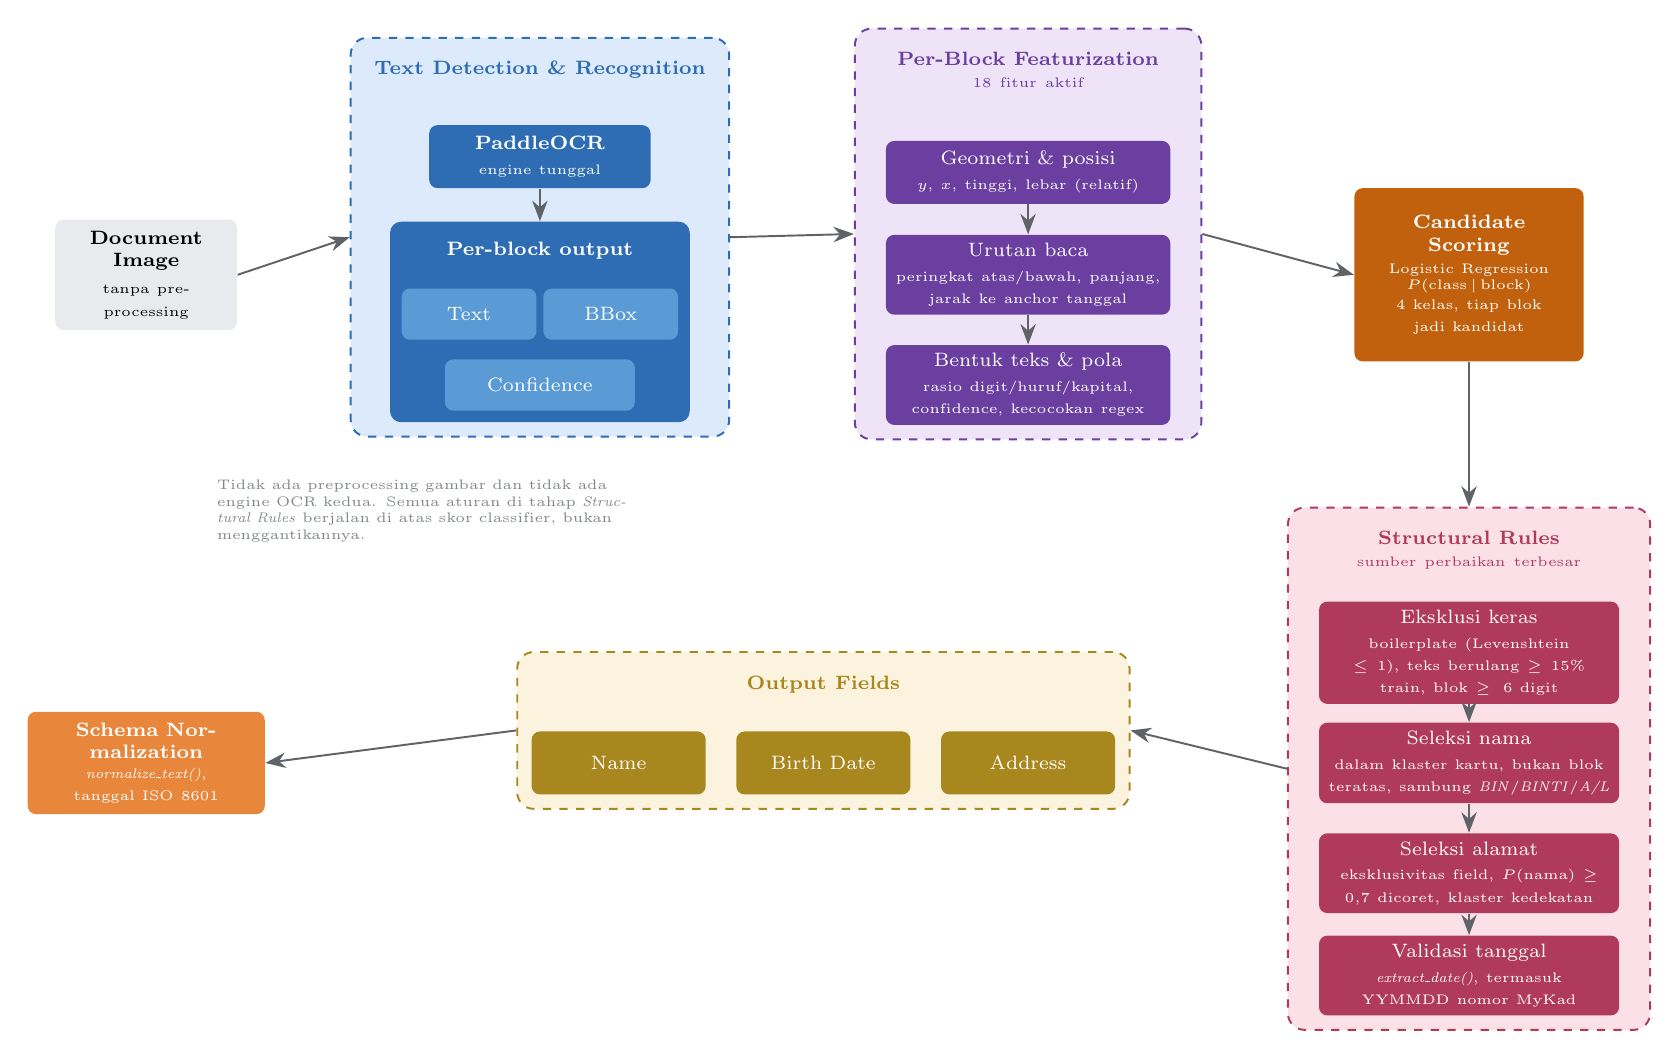
\begin{tikzpicture}[
  x=1mm, y=1mm, font=\scriptsize,
  blk/.style={rounded corners=3pt, draw=none, align=center, text=white,
              inner sep=3pt, minimum height=8mm, text width=24mm},
  grp/.style={rounded corners=6pt, dashed, line width=0.7pt, inner sep=5pt},
  lbl/.style={font=\scriptsize\bfseries, align=center},
  ar/.style={-{Stealth[length=2.6mm]}, draw=gEdge, line width=0.7pt},
]

% ============================================================ ROW 1
% ---- 1. input
\node[blk, fill=gGray, text=black, text width=21mm, minimum height=14mm] at (0,0) (img)
  {\textbf{Document}\\\textbf{Image}\\[2pt]{\tiny tanpa preprocessing}};

% ---- 2. OCR
\node[blk, fill=gBlue, text width=26mm] at (50,15) (ocr)
  {\textbf{PaddleOCR}\\[1pt]{\tiny engine tunggal}};
\node[lbl, text=white] at (50,3) (exl) {Per-block output};
\node[blk, fill=gBlueLt, text width=15mm, minimum height=6.5mm] at (41,-5) (txt) {Text};
\node[blk, fill=gBlueLt, text width=15mm, minimum height=6.5mm] at (59,-5) (bbx) {BBox};
\node[blk, fill=gBlueLt, text width=22mm, minimum height=6.5mm] at (50,-14) (cnf) {Confidence};
\begin{pgfonlayer}{bgA}
  \node[rounded corners=4pt, fill=gBlue, inner sep=4pt, fit=(exl)(txt)(bbx)(cnf)] (extbox) {};
\end{pgfonlayer}
\node[lbl, text=gBlue] at (50,26) (fel) {Text Detection \& Recognition};
\begin{pgfonlayer}{bgB}
  \node[grp, draw=gBlue, fill=gBlueBg, fit=(fel)(ocr)(extbox)] (gA) {};
\end{pgfonlayer}

% ---- 3. per-block featurization
\node[blk, fill=gPur, text width=34mm] at (112,13) (s1)
  {Geometri \& posisi\\[1pt]{\tiny $y$, $x$, tinggi, lebar (relatif)}};
\node[blk, fill=gPur, text width=34mm] at (112,0) (s2)
  {Urutan baca\\[1pt]{\tiny peringkat atas/bawah, panjang, jarak ke anchor tanggal}};
\node[blk, fill=gPur, text width=34mm] at (112,-14) (s3)
  {Bentuk teks \& pola\\[1pt]{\tiny rasio digit/huruf/kapital, confidence, kecocokan regex}};
\node[lbl, text=gPur, text width=38mm] at (112,26) (sl) {Per-Block Featurization\\{\tiny\mdseries 18 fitur aktif}};
\begin{pgfonlayer}{bgB}
  \node[grp, draw=gPur, fill=gPurBg, fit=(sl)(s1)(s2)(s3)] (gB) {};
\end{pgfonlayer}

% ---- 4. classifier
\node[blk, fill=gOrange, text width=27mm, minimum height=22mm] at (168,0) (cand)
  {\textbf{Candidate}\\\textbf{Scoring}\\[2pt]{\tiny Logistic Regression\\$P(\mathrm{class}\,|\,\mathrm{block})$\\[1pt]4 kelas, tiap blok\\jadi kandidat}};

% ============================================================ ROW 2
% ---- 5. structural rules
\node[blk, fill=gPink, text width=36mm] at (168,-48) (r1)
  {Eksklusi keras\\[1pt]{\tiny boilerplate (Levenshtein $\leq 1$), teks berulang $\geq 15\%$ train, blok $\geq 6$ digit}};
\node[blk, fill=gPink, text width=36mm] at (168,-62) (r2)
  {Seleksi nama\\[1pt]{\tiny dalam klaster kartu, bukan blok teratas, sambung \textit{BIN}/\textit{BINTI}/\textit{A/L}}};
\node[blk, fill=gPink, text width=36mm] at (168,-76) (r3)
  {Seleksi alamat\\[1pt]{\tiny eksklusivitas field, $P(\mathrm{nama}) \geq 0{,}7$ dicoret, klaster kedekatan}};
\node[blk, fill=gPink, text width=36mm] at (168,-89) (r4)
  {Validasi tanggal\\[1pt]{\tiny \textit{extract\_date()}, termasuk YYMMDD nomor MyKad}};
\node[lbl, text=gPink, text width=40mm] at (168,-35) (rl) {Structural Rules\\{\tiny\mdseries sumber perbaikan terbesar}};
\begin{pgfonlayer}{bgB}
  \node[grp, draw=gPink, fill=gPinkBg, fit=(rl)(r1)(r2)(r3)(r4)] (gC) {};
\end{pgfonlayer}

% ---- 6. output fields
\node[blk, fill=gTan, text width=20mm] at (60,-62)  (fname) {Name};
\node[blk, fill=gTan, text width=20mm] at (86,-62)  (fbod)  {Birth Date};
\node[blk, fill=gTan, text width=20mm] at (112,-62) (faddr) {Address};
\node[lbl, text=gTan] at (86,-52) (ol) {Output Fields};
\begin{pgfonlayer}{bgB}
  \node[grp, draw=gTan, fill=gCream, fit=(ol)(fname)(fbod)(faddr)] (gD) {};
\end{pgfonlayer}

% ---- 7. normalization
\node[blk, fill=gAmber, text width=28mm, minimum height=13mm] at (0,-62) (norm)
  {\textbf{Schema Normalization}\\[1pt]{\tiny \textit{normalize\_text()},\\tanggal ISO 8601}};

% ============================================================ arrows
\draw[ar] (img.east)   -- (gA.west);
\draw[ar] (ocr.south)  -- (extbox.north);
\draw[ar] (gA.east)    -- (gB.west);
\draw[ar] (gB.east)    -- (cand.west);
\draw[ar] (cand.south) -- (gC.north);
\draw[ar] (gC.west)    -- (gD.east);
\draw[ar] (gD.west)    -- (norm.east);
\draw[ar] (s1) -- (s2);
\draw[ar] (s2) -- (s3);
\draw[ar] (r1) -- (r2);
\draw[ar] (r2) -- (r3);
\draw[ar] (r3) -- (r4);

% catatan
\node[align=left, text=gMuted, font=\tiny, text width=52mm] at (35,-30)
  {Tidak ada preprocessing gambar dan tidak ada engine OCR kedua.
   Semua aturan di tahap \textit{Structural Rules} berjalan di atas skor
   classifier, bukan menggantikannya.};

\end{tikzpicture}
\end{document}
